\documentclass[12pt, a4paper]{article}
% Some fancy symbols
\usepackage{textcomp}
\usepackage{stmaryrd}
\usepackage{cancel}

% Some fancy symbols
\usepackage{textcomp}
\usepackage{stmaryrd}


\usepackage{array}

% Math packages
\usepackage{amsmath,amsthm,amssymb, amsfonts, mathrsfs, dsfont, mathtools}
% \usepackage{mathtext}

\usepackage[bb=boondox]{mathalfa}
\usepackage{bm}

% To conrol figures:
\usepackage{subfig}
\usepackage{adjustbox}
\usepackage{placeins}
\usepackage{rotating}



\usepackage{lipsum}
\usepackage{psvectorian} % Insanely fancy text separators!


% Refs:
\usepackage{url}
\usepackage[backref]{hyperref}

% Fancier tables and lists
\usepackage{booktabs}
\usepackage{enumitem}
% Don't indent paragraphs, leave some space between them
\usepackage{parskip}
% Hide page number when page is empty
\usepackage{emptypage}


\usepackage{multicol}
\usepackage{xcolor}

\usepackage[normalem]{ulem}

% For beautiful code listings:
% \usepackage{minted}
\usepackage{listings}

\usepackage{csquotes} % For citations
\usepackage[framemethod=tikz]{mdframed} % For further information see: http://marcodaniel.github.io/mdframed/

% Plots
\usepackage{pgfplots} 
\pgfplotsset{width=10cm,compat=1.9} 

% Fonts
\usepackage{unicode-math}
% \setmathfont{TeX Gyre Termes Math}

\usepackage{fontspec}
\usepackage{polyglossia}

% Named references to sections in document:
\usepackage{nameref}


% \setmainfont{Times New Roman}
\setdefaultlanguage{russian}

\newfontfamily\cyrillicfont{Kurale}
\setmainfont[Ligatures=TeX]{Kurale}
\setmonofont{Fira Code}

% Common number sets
\newcommand{\sN}{{\mathbb{N}}}
\newcommand{\sZ}{{\mathbb{Z}}}
\newcommand{\sZp}{{\mathbb{Z}^{+}}}
\newcommand{\sQ}{{\mathbb{Q}}}
\newcommand{\sR}{{\mathbb{R}}}
\newcommand{\sRp}{{\mathbb{R^{+}}}}
\newcommand{\sC}{{\mathbb{C}}}
\newcommand{\sB}{{\mathbb{B}}}

% Math operators

\makeatletter
\newcommand\RedeclareMathOperator{%
  \@ifstar{\def\rmo@s{m}\rmo@redeclare}{\def\rmo@s{o}\rmo@redeclare}%
}
% this is taken from \renew@command
\newcommand\rmo@redeclare[2]{%
  \begingroup \escapechar\m@ne\xdef\@gtempa{{\string#1}}\endgroup
  \expandafter\@ifundefined\@gtempa
     {\@latex@error{\noexpand#1undefined}\@ehc}%
     \relax
  \expandafter\rmo@declmathop\rmo@s{#1}{#2}}
% This is just \@declmathop without \@ifdefinable
\newcommand\rmo@declmathop[3]{%
  \DeclareRobustCommand{#2}{\qopname\newmcodes@#1{#3}}%
}
\@onlypreamble\RedeclareMathOperator
\makeatother


% Correction:
\definecolor{correct_color}{HTML}{009900}
\newcommand\correction[2]{\ensuremath{\:}{\color{red}{#1}}\ensuremath{\to }{\color{correct_color}{#2}}\ensuremath{\:}}
\newcommand\inGreen[1]{{\color{correct_color}{#1}}}

% Roman numbers && fancy symbs:
\newcommand{\RNumb}[1]{{\uppercase\expandafter{\romannumeral #1\relax}}}
\newcommand\textbb[1]{{$\mathbb{#1}$}}



% MD framed environments:
\mdfsetup{skipabove=1em,skipbelow=0em}

% \mdfdefinestyle{definition}{%
%     linewidth=2pt,%
%     frametitlebackgroundcolor=white,
%     % innertopmargin=\topskip,
% }

\theoremstyle{definition}
\newmdtheoremenv[nobreak=true]{definition}{Определение}
\newmdtheoremenv[nobreak=true]{theorem}{Теорема}
\newmdtheoremenv[nobreak=true]{lemma}{Лемма}
\newmdtheoremenv[nobreak=true]{problem}{Задача}
\newmdtheoremenv[nobreak=true]{property}{Свойство}
\newmdtheoremenv[nobreak=true]{statement}{Утверждение}
\newmdtheoremenv[nobreak=true]{corollary}{Следствие}
\newtheorem*{note}{Замечание}
\newtheorem*{example}{Пример}

% To mark logical parts
\newcommand{\existence}{{\circled{$\exists$}}}
\newcommand{\uniqueness}{{\circled{$\hspace{0.5px}!$}}}
\newcommand{\rightimp}{{\circled{$\Rightarrow$}}}
\newcommand{\leftimp}{{\circled{$\Leftarrow$}}}


% Useful symbols:
\renewcommand{\qed}{\ensuremath{\blacksquare}}
\renewcommand{\vec}[1]{\overrightarrow{#1}}
\newcommand{\eqdef}{\overset{\mathrm{def}}{=\joinrel=}}
\newcommand{\isdef}{\overset{\mathrm{def}}{\Longleftrightarrow}}
\newcommand{\inductdots}{\ensuremath{\overset{induction}{\cdots}}}

% Matrix's determinant
\newenvironment{detmatrix}
{
  \left|\begin{matrix}
}{
  \end{matrix}\right|
}

\newenvironment{complex}
{
  \left[\begin{gathered}
}{
  \end{gathered}\right.
}


\newcommand{\nl}{$~$\\}

\newcommand{\tit}{\maketitle\newpage}
\newcommand{\tittoc}{\tit\tableofcontents\newpage}


\newcommand{\vova}{  
    Латыпов Владимир (конспектор)\\
    {\small \texttt{t.me/donRumata03}, \texttt{github.com/donRumata03}, \texttt{donrumata03@gmail.com}}
}


\usepackage{tikz}
\newcommand{\circled}[1]{\tikz[baseline=(char.base)]{
            \node[shape=circle,draw,inner sep=2pt] (char) {#1};}}

\newcommand{\contradiction}{\circled{!!!}}

% Make especially big math:

\makeatletter
\newcommand{\biggg}{\bBigg@\thr@@}
\newcommand{\Biggg}{\bBigg@{4.5}}
\def\bigggl{\mathopen\biggg}
\def\bigggm{\mathrel\biggg}
\def\bigggr{\mathclose\biggg}
\def\Bigggl{\mathopen\Biggg}
\def\Bigggm{\mathrel\Biggg}
\def\Bigggr{\mathclose\Biggg}
\makeatother


% Texts dividers:

\newcommand{\ornamentleft}{%
    \psvectorian[width=2em]{2}%
}
\newcommand{\ornamentright}{%
    \psvectorian[width=2em,mirror]{2}%
}
\newcommand{\ornamentbreak}{%
    \begin{center}
    \ornamentleft\quad\ornamentright
    \end{center}%
}
\newcommand{\ornamentheader}[1]{%
    \begin{center}
    \ornamentleft
    \quad{\large\emph{#1}}\quad % style as desired
    \ornamentright
    \end{center}%
}


% Math operators

\DeclareMathOperator{\sgn}{sgn}
\DeclareMathOperator{\id}{id}
\DeclareMathOperator{\rg}{rg}
\DeclareMathOperator{\determinant}{det}

\DeclareMathOperator{\Aut}{Aut}

\DeclareMathOperator{\Sim}{Sim}
\DeclareMathOperator{\Alt}{Alt}



\DeclareMathOperator{\Int}{Int}
\DeclareMathOperator{\Cl}{Cl}
\DeclareMathOperator{\Ext}{Ext}
\DeclareMathOperator{\Fr}{Fr}


\RedeclareMathOperator{\Re}{Re}
\RedeclareMathOperator{\Im}{Im}


\DeclareMathOperator{\Img}{Im}
\DeclareMathOperator{\Ker}{Ker}
\DeclareMathOperator{\Lin}{Lin}
\DeclareMathOperator{\Span}{span}

\DeclareMathOperator{\tr}{tr}
\DeclareMathOperator{\conj}{conj}
\DeclareMathOperator{\diag}{diag}

\expandafter\let\expandafter\originald\csname\encodingdefault\string\d\endcsname
\DeclareRobustCommand*\d
  {\ifmmode\mathop{}\!\mathrm{d}\else\expandafter\originald\fi}

\newcommand\restr[2]{{% we make the whole thing an ordinary symbol
  \left.\kern-\nulldelimiterspace % automatically resize the bar with \right
  #1 % the function
  \vphantom{\big|} % pretend it's a little taller at normal size
  \right|_{#2} % this is the delimiter
  }}

\newcommand{\splitdoc}{\noindent\makebox[\linewidth]{\rule{\paperwidth}{0.4pt}}}

% \newcommand{\hm}[1]{#1\nobreak\discretionary{}{\hbox{\ensuremath{#1}}}{}}


\usepackage{geometry}
\geometry{
    a4paper,
    left=30mm,
    right=30mm,
    top=30mm,
    bottom=20mm
}


\author{Латыпов Владимир Витальевич, \\ ИТМО КТ M3138, \Huge{\textit{\textbf{вариант 12}}}}
\title{Типовик по линейной алгебре модуль 1: Задание 6 «Кривые второго порядка»}

\begin{document}
    \tittoc

    \section{Формулировка условия}

    \begin{statement}
        Условие таково: 
        
        12. Оси гиперболы совпадают с осями координат. Гипербола проходит
        через точки пересечения параболы $x^2 = 2y$ с прямой $x − 2y + 6 = 0$.
        
        Составить уравнение этой гиперболы.

        Сделать рисунок.
    \end{statement}

    \section{Решение}

    \ornamentheader{Что исправлено? Раньше не учитывалось, что, исходя из формулировки задачи оси гиперболы могут «совпадать с осями координат» двумя разными способами}

    Для начала найдём эти точки пересечения, решив квадратное уравнение (для обоих случаев они совпадают):
    \begin{gather}
        \begin{cases}
            x^2 = 2y \\
            x − 2y + 6 = 0
        \end{cases} \\
        \begin{cases}
            y = \frac{x^2}{2} \\
            x − 2\cdot \frac{x^2}{2} + 6 = 0
        \end{cases} \\
        x^2 - x - 6 = 0 \\
        \begin{complex}
            x = -2, y = \frac{2^2}{2} = 2 \\
            x = 3, y = \frac{3^2}{2} = 4.5
        \end{complex}
    \end{gather}

    То есть гипербола должна проходить через точки $(-2, 2)$ и $(3, 4.5)$.

    У параболы, указанной в условии, остаётся только два параметра — главная и мнимая полуоси.
    Причём есть два варианта их ориертации: \begin{enumerate}
        \item Главная полуось совпадает с осью $OX$, минимая — с осью $OY$.
        \item Наоборот: Главная полуось совпадает с осью $OY$, минимая — с осью $OX$.
    \end{enumerate}.

    Рассмотрим оба случая.

    \subsection{Случай 1}

    Найдём их значения, потребовав, что гипербола проходит там, где надо.

    \begin{gather}
        \begin{cases}
            \frac{(-2)^2}{a^2} - \frac{2^2}{b^2} = 1 \\
            \frac{3^2}{a^2} - \frac{\left(\frac{9}{2}\right)^2}{b^2} = 1
        \end{cases}
    \end{gather}

    За $\alpha$ обозначим $a^2$, за $\beta$ — $b^2$, помним, что оба параметра больше нуля.

    \begin{gather}
        \begin{cases}
            4\beta - 4\alpha = \alpha\beta \\
            9\beta - \frac{81}{4} \alpha = \alpha\beta
        \end{cases} \\
        4\beta - 4\alpha = 9\beta - \frac{81}{4} \alpha \\
        \frac{65}{4}\alpha = 5\beta \\
        \beta = \frac{13}{4}\alpha \\
        4 \left( \frac{13}{4}\alpha \right) - 4\alpha = \alpha \cdot \frac{13}{4}\alpha \\
        13 - 4 = \frac{13}{4}\alpha \Longrightarrow \alpha = \frac{9 \cdot 4}{13} \Longrightarrow a = \sqrt{\alpha} = \frac{6}{\sqrt{13}} \\
        \beta = \frac{13}{4}\alpha = \frac{\cancel{13}}{\cancel{4}} \cdot \frac{9 \cdot \cancel{4}}{\cancel{13}} = 9 \Longrightarrow b = \sqrt{\beta} = 3
    \end{gather}

    Таким образом, уравнение гиперболы в этом случае:
    \begin{equation}
        \frac{13}{36} x^2 - \frac{y^2}{9} = 1
    \end{equation}


    \subsection{Случай 2}

    Аналогичные уравнения, но с переменой главной и мнимой полуосей местами 
    гарантируют нам прохождение через точки пересечения:
    
    \begin{gather}
        \begin{cases}
            \frac{(-2)^2}{b^2} - \frac{2^2}{a^2} = 1 \\
            \frac{3^2}{b^2} - \frac{\left(\frac{9}{2}\right)^2}{a^2} = 1
        \end{cases}
    \end{gather}

    Всё ещё за $\alpha$ обозначим $a^2$, за $\beta$ — $b^2$. И всё ещё помним, что оба параметра больше нуля.

    \begin{gather}
        \begin{cases}
            4\alpha - 4\beta = \alpha\beta \\
            9\alpha - \frac{81}{4} \beta = \alpha\beta
        \end{cases} \\
        4\alpha - 4\beta = 9\alpha - \frac{81}{4} \beta \\
        \beta \left( \frac{81}{4} - 4 \right) = 5\alpha \\
        \beta \left( \frac{65}{4} \right) = 5\alpha \\
        \begin{cases}
            \alpha = \beta \left( \frac{65}{20} \right) \\
            4\alpha - 4\beta = \alpha\beta
        \end{cases} \\
        \begin{cases}
            \alpha = \beta \left( \frac{65}{20} \right) \\
            4 \cancel{\beta} \left( \frac{65}{20} \right) - 4\cancel{\beta} = \cancel{\beta} \left( \frac{65}{20} \right)\beta
        \end{cases} \\
        4 \left( \frac{65}{20} \right) - 4 = \frac{65}{20} \beta \\
        \beta = \frac{4 \left( \frac{65}{20} \right) - 4}{\frac{65}{20}} = \frac{36}{13} \\
        \alpha = \frac{65}{20} \times \frac{36}{13} = 9
    \end{gather}

    Кто бы мог подумать: мы решили то же уравнение, только с $\alpha$ и $\beta$ изменёнными местами.
    И получили тот же самый ответ. Следовательно, он уж точно верный.

    Соответственно, уравнение второй гиперболы:
    \begin{equation}
        \frac{13}{36} y^2 - \frac{x^2}{9} = 1
    \end{equation}


    \section{Иллюстрация}
    
    (здесь будет нарисован чертёж)
    

    \begin{figure}[h!]
        \centering
        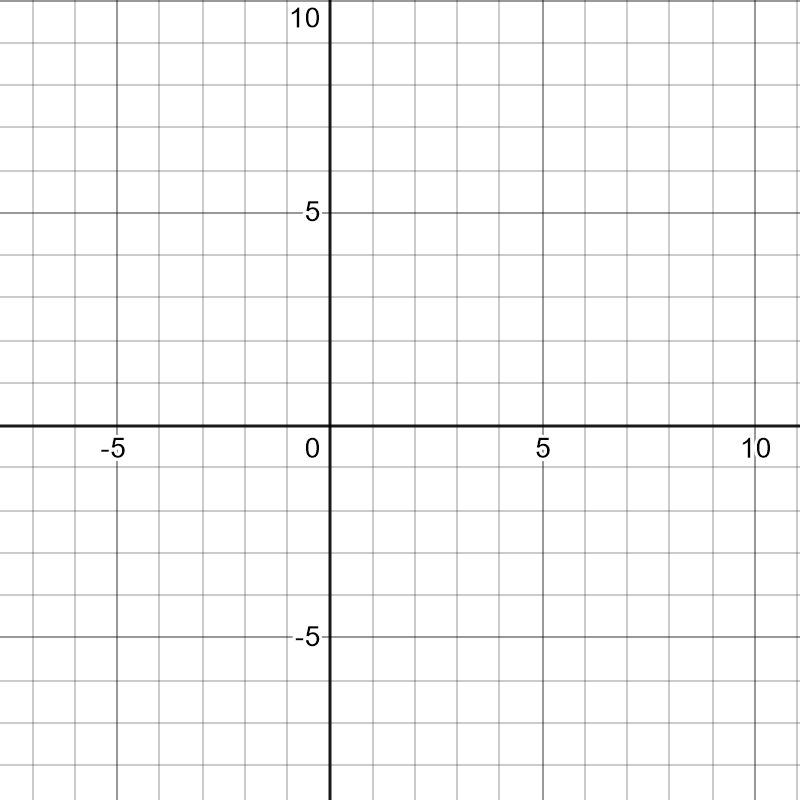
\includegraphics[width=\textwidth]{resources/1.6_grid.png}
        \caption{Чертёж}
        \label{fig:main_figure}
    \end{figure}
    \FloatBarrier


\end{document}
